\documentclass[12pt]{article}
\usepackage[margin=1.0in]{geometry}
\usepackage[utf8]{inputenc}
\usepackage[T1]{fontenc}
\usepackage{lmodern}
\usepackage[spanish]{babel}
\usepackage{amsmath}
\usepackage{graphicx}

\title{Response to the referee}

\begin{document}

\date{}
\maketitle

\section*{Outflow + Rotation}

We want to study the pure effect of rotation on the spectra, off course it would
be interesting to study the effect of rotation on systems with outflows, this paper
is under preparation by M.C Remolina-Gutierrez et al.  

\section*{Details}

\subsection*{Introduction}

This changes were performed.

\subsection*{Fig.1}

\begin{itemize}
\item Description about how we build Fig.1 (Done)
\item Fig 1. remove x notation (Done)
\end{itemize}

\subsection*{Fig.2}

Explanation (Done)\\
We don't fit a gaussian , we measure the width by finding
the closest points to the half maximum in our histogram numerically.

\subsection*{Fig.3}



\subsection*{Fig4 and 6}

Waiting for the cluster in germany!

\subsection*{Fig5}
\begin{figure}
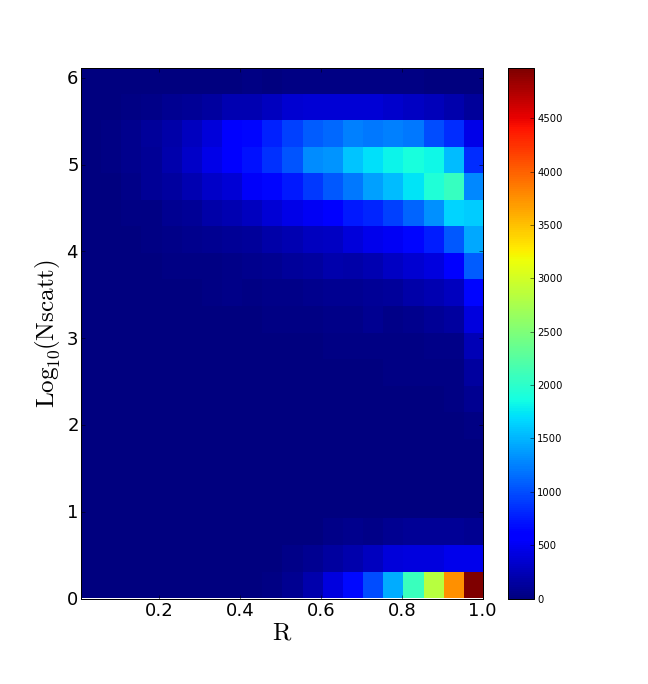
\includegraphics[scale=0.4]{Histogram2dNscattVSRadius.png}
\end{figure}

\end{document}